
\newsavebox{\boxshapea}
\sbox{\boxshapea}{
  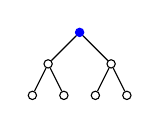
\begin{tikzpicture}[baseline=-0.5ex, scale=0.4]
    \tikzset{every node/.style={draw, circle, inner sep=0.5pt, minimum size=3pt}}
    \node[] (N4) at (-1.50, -2) {};
    \node[] (N5) at (-0.50, -2) {};
    \node[] (N2) at (-1.00, -1) {};
    \node[] (N6) at (0.50, -2) {};
    \node[] (N7) at (1.50, -2) {};
    \node[] (N3) at (1.00, -1) {};
    \node[fill=Blue, draw=Blue] (N1) at (0.00, 0) {};
    \draw (N1) -- (N2);
    \draw (N2) -- (N4);
    \draw (N2) -- (N5);
    \draw (N1) -- (N3);
    \draw (N3) -- (N6);
    \draw (N3) -- (N7);
  \end{tikzpicture}
}
\newsavebox{\boxshapeb}
\sbox{\boxshapeb}{
  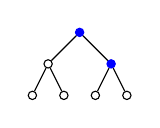
\begin{tikzpicture}[baseline=-0.5ex, scale=0.4]
    \tikzset{every node/.style={draw, circle, inner sep=0.5pt, minimum size=3pt}}
    \node[] (N4) at (-1.50, -2) {};
    \node[] (N5) at (-0.50, -2) {};
    \node[] (N2) at (-1.00, -1) {};
    \node[] (N6) at (0.50, -2) {};
    \node[] (N7) at (1.50, -2) {};
    \node[fill=Blue, draw=Blue] (N3) at (1.00, -1) {};
    \node[fill=Blue, draw=Blue] (N1) at (0.00, 0) {};
    \draw (N1) -- (N2);
    \draw (N2) -- (N4);
    \draw (N2) -- (N5);
    \draw (N1) -- (N3);
    \draw (N3) -- (N6);
    \draw (N3) -- (N7);
  \end{tikzpicture}
}
\newsavebox{\boxshapec}
\sbox{\boxshapec}{
  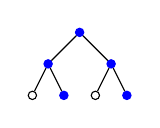
\begin{tikzpicture}[baseline=-0.5ex, scale=0.4]
    \tikzset{every node/.style={draw, circle, inner sep=0.5pt, minimum size=3pt}}
    \node[] (N4) at (-1.50, -2) {};
    \node[fill=Blue, draw=Blue] (N5) at (-0.50, -2) {};
    \node[fill=Blue, draw=Blue] (N2) at (-1.00, -1) {};
    \node[] (N6) at (0.50, -2) {};
    \node[fill=Blue, draw=Blue] (N7) at (1.50, -2) {};
    \node[fill=Blue, draw=Blue] (N3) at (1.00, -1) {};
    \node[fill=Blue, draw=Blue] (N1) at (0.00, 0) {};
    \draw (N1) -- (N2);
    \draw (N2) -- (N4);
    \draw (N2) -- (N5);
    \draw (N1) -- (N3);
    \draw (N3) -- (N6);
    \draw (N3) -- (N7);
  \end{tikzpicture}
}
\newsavebox{\boxshaped}
\sbox{\boxshaped}{
  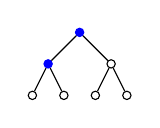
\begin{tikzpicture}[baseline=-0.5ex, scale=0.4]
    \tikzset{every node/.style={draw, circle, inner sep=0.5pt, minimum size=3pt}}
    \node[] (N4) at (-1.50, -2) {};
    \node[] (N5) at (-0.50, -2) {};
    \node[fill=Blue, draw=Blue] (N2) at (-1.00, -1) {};
    \node[] (N6) at (0.50, -2) {};
    \node[] (N7) at (1.50, -2) {};
    \node[] (N3) at (1.00, -1) {};
    \node[fill=Blue, draw=Blue] (N1) at (0.00, 0) {};
    \draw (N1) -- (N2);
    \draw (N2) -- (N4);
    \draw (N2) -- (N5);
    \draw (N1) -- (N3);
    \draw (N3) -- (N6);
    \draw (N3) -- (N7);
  \end{tikzpicture}
}
\newsavebox{\boxshapee}
\sbox{\boxshapee}{
  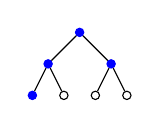
\begin{tikzpicture}[baseline=-0.5ex, scale=0.4]
    \tikzset{every node/.style={draw, circle, inner sep=0.5pt, minimum size=3pt}}
    \node[fill=Blue, draw=Blue] (N4) at (-1.50, -2) {};
    \node[] (N5) at (-0.50, -2) {};
    \node[fill=Blue, draw=Blue] (N2) at (-1.00, -1) {};
    \node[] (N6) at (0.50, -2) {};
    \node[] (N7) at (1.50, -2) {};
    \node[fill=Blue, draw=Blue] (N3) at (1.00, -1) {};
    \node[fill=Blue, draw=Blue] (N1) at (0.00, 0) {};
    \draw (N1) -- (N2);
    \draw (N2) -- (N4);
    \draw (N2) -- (N5);
    \draw (N1) -- (N3);
    \draw (N3) -- (N6);
    \draw (N3) -- (N7);
  \end{tikzpicture}
}
\newsavebox{\boxshapef}
\sbox{\boxshapef}{
  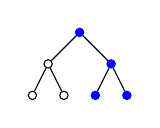
\begin{tikzpicture}[baseline=-0.5ex, scale=0.4]
    \tikzset{every node/.style={draw, circle, inner sep=0.5pt, minimum size=3pt}}
    \node[] (N4) at (-1.50, -2) {};
    \node[] (N5) at (-0.50, -2) {};
    \node[] (N2) at (-1.00, -1) {};
    \node[fill=Blue, draw=Blue] (N6) at (0.50, -2) {};
    \node[fill=Blue, draw=Blue] (N7) at (1.50, -2) {};
    \node[fill=Blue, draw=Blue] (N3) at (1.00, -1) {};
    \node[fill=Blue, draw=Blue] (N1) at (0.00, 0) {};
    \draw (N1) -- (N2);
    \draw (N2) -- (N4);
    \draw (N2) -- (N5);
    \draw (N1) -- (N3);
    \draw (N3) -- (N6);
    \draw (N3) -- (N7);
  \end{tikzpicture}
}
\newsavebox{\boxshapeg}
\sbox{\boxshapeg}{
  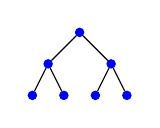
\begin{tikzpicture}[baseline=-0.5ex, scale=0.4]
    \tikzset{every node/.style={draw, circle, inner sep=0.5pt, minimum size=3pt}}
    \node[fill=Blue, draw=Blue] (N4) at (-1.50, -2) {};
    \node[fill=Blue, draw=Blue] (N5) at (-0.50, -2) {};
    \node[fill=Blue, draw=Blue] (N2) at (-1.00, -1) {};
    \node[fill=Blue, draw=Blue] (N6) at (0.50, -2) {};
    \node[fill=Blue, draw=Blue] (N7) at (1.50, -2) {};
    \node[fill=Blue, draw=Blue] (N3) at (1.00, -1) {};
    \node[fill=Blue, draw=Blue] (N1) at (0.00, 0) {};
    \draw (N1) -- (N2);
    \draw (N2) -- (N4);
    \draw (N2) -- (N5);
    \draw (N1) -- (N3);
    \draw (N3) -- (N6);
    \draw (N3) -- (N7);
  \end{tikzpicture}
}
\newsavebox{\boxshapeh}
\sbox{\boxshapeh}{
  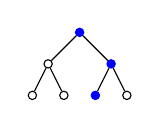
\begin{tikzpicture}[baseline=-0.5ex, scale=0.4]
    \tikzset{every node/.style={draw, circle, inner sep=0.5pt, minimum size=3pt}}
    \node[] (N4) at (-1.50, -2) {};
    \node[] (N5) at (-0.50, -2) {};
    \node[] (N2) at (-1.00, -1) {};
    \node[fill=Blue, draw=Blue] (N6) at (0.50, -2) {};
    \node[] (N7) at (1.50, -2) {};
    \node[fill=Blue, draw=Blue] (N3) at (1.00, -1) {};
    \node[fill=Blue, draw=Blue] (N1) at (0.00, 0) {};
    \draw (N1) -- (N2);
    \draw (N2) -- (N4);
    \draw (N2) -- (N5);
    \draw (N1) -- (N3);
    \draw (N3) -- (N6);
    \draw (N3) -- (N7);
  \end{tikzpicture}
}
\newsavebox{\boxshapei}
\sbox{\boxshapei}{
  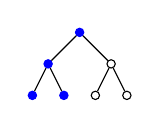
\begin{tikzpicture}[baseline=-0.5ex, scale=0.4]
    \tikzset{every node/.style={draw, circle, inner sep=0.5pt, minimum size=3pt}}
    \node[fill=Blue, draw=Blue] (N4) at (-1.50, -2) {};
    \node[fill=Blue, draw=Blue] (N5) at (-0.50, -2) {};
    \node[fill=Blue, draw=Blue] (N2) at (-1.00, -1) {};
    \node[] (N6) at (0.50, -2) {};
    \node[] (N7) at (1.50, -2) {};
    \node[] (N3) at (1.00, -1) {};
    \node[fill=Blue, draw=Blue] (N1) at (0.00, 0) {};
    \draw (N1) -- (N2);
    \draw (N2) -- (N4);
    \draw (N2) -- (N5);
    \draw (N1) -- (N3);
    \draw (N3) -- (N6);
    \draw (N3) -- (N7);
  \end{tikzpicture}
}
\newsavebox{\boxshapej}
\sbox{\boxshapej}{
  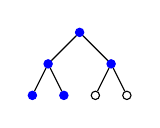
\begin{tikzpicture}[baseline=-0.5ex, scale=0.4]
    \tikzset{every node/.style={draw, circle, inner sep=0.5pt, minimum size=3pt}}
    \node[fill=Blue, draw=Blue] (N4) at (-1.50, -2) {};
    \node[fill=Blue, draw=Blue] (N5) at (-0.50, -2) {};
    \node[fill=Blue, draw=Blue] (N2) at (-1.00, -1) {};
    \node[] (N6) at (0.50, -2) {};
    \node[] (N7) at (1.50, -2) {};
    \node[fill=Blue, draw=Blue] (N3) at (1.00, -1) {};
    \node[fill=Blue, draw=Blue] (N1) at (0.00, 0) {};
    \draw (N1) -- (N2);
    \draw (N2) -- (N4);
    \draw (N2) -- (N5);
    \draw (N1) -- (N3);
    \draw (N3) -- (N6);
    \draw (N3) -- (N7);
  \end{tikzpicture}
}
\newsavebox{\boxshapek}
\sbox{\boxshapek}{
  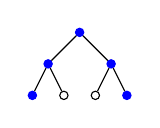
\begin{tikzpicture}[baseline=-0.5ex, scale=0.4]
    \tikzset{every node/.style={draw, circle, inner sep=0.5pt, minimum size=3pt}}
    \node[fill=Blue, draw=Blue] (N4) at (-1.50, -2) {};
    \node[] (N5) at (-0.50, -2) {};
    \node[fill=Blue, draw=Blue] (N2) at (-1.00, -1) {};
    \node[] (N6) at (0.50, -2) {};
    \node[fill=Blue, draw=Blue] (N7) at (1.50, -2) {};
    \node[fill=Blue, draw=Blue] (N3) at (1.00, -1) {};
    \node[fill=Blue, draw=Blue] (N1) at (0.00, 0) {};
    \draw (N1) -- (N2);
    \draw (N2) -- (N4);
    \draw (N2) -- (N5);
    \draw (N1) -- (N3);
    \draw (N3) -- (N6);
    \draw (N3) -- (N7);
  \end{tikzpicture}
}
\newsavebox{\boxshapel}
\sbox{\boxshapel}{
  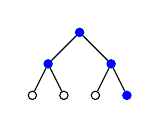
\begin{tikzpicture}[baseline=-0.5ex, scale=0.4]
    \tikzset{every node/.style={draw, circle, inner sep=0.5pt, minimum size=3pt}}
    \node[] (N4) at (-1.50, -2) {};
    \node[] (N5) at (-0.50, -2) {};
    \node[fill=Blue, draw=Blue] (N2) at (-1.00, -1) {};
    \node[] (N6) at (0.50, -2) {};
    \node[fill=Blue, draw=Blue] (N7) at (1.50, -2) {};
    \node[fill=Blue, draw=Blue] (N3) at (1.00, -1) {};
    \node[fill=Blue, draw=Blue] (N1) at (0.00, 0) {};
    \draw (N1) -- (N2);
    \draw (N2) -- (N4);
    \draw (N2) -- (N5);
    \draw (N1) -- (N3);
    \draw (N3) -- (N6);
    \draw (N3) -- (N7);
  \end{tikzpicture}
}
\newsavebox{\boxshapem}
\sbox{\boxshapem}{
  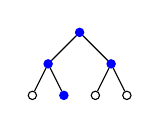
\begin{tikzpicture}[baseline=-0.5ex, scale=0.4]
    \tikzset{every node/.style={draw, circle, inner sep=0.5pt, minimum size=3pt}}
    \node[] (N4) at (-1.50, -2) {};
    \node[fill=Blue, draw=Blue] (N5) at (-0.50, -2) {};
    \node[fill=Blue, draw=Blue] (N2) at (-1.00, -1) {};
    \node[] (N6) at (0.50, -2) {};
    \node[] (N7) at (1.50, -2) {};
    \node[fill=Blue, draw=Blue] (N3) at (1.00, -1) {};
    \node[fill=Blue, draw=Blue] (N1) at (0.00, 0) {};
    \draw (N1) -- (N2);
    \draw (N2) -- (N4);
    \draw (N2) -- (N5);
    \draw (N1) -- (N3);
    \draw (N3) -- (N6);
    \draw (N3) -- (N7);
  \end{tikzpicture}
}
\newsavebox{\boxshapen}
\sbox{\boxshapen}{
  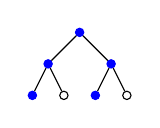
\begin{tikzpicture}[baseline=-0.5ex, scale=0.4]
    \tikzset{every node/.style={draw, circle, inner sep=0.5pt, minimum size=3pt}}
    \node[fill=Blue, draw=Blue] (N4) at (-1.50, -2) {};
    \node[] (N5) at (-0.50, -2) {};
    \node[fill=Blue, draw=Blue] (N2) at (-1.00, -1) {};
    \node[fill=Blue, draw=Blue] (N6) at (0.50, -2) {};
    \node[] (N7) at (1.50, -2) {};
    \node[fill=Blue, draw=Blue] (N3) at (1.00, -1) {};
    \node[fill=Blue, draw=Blue] (N1) at (0.00, 0) {};
    \draw (N1) -- (N2);
    \draw (N2) -- (N4);
    \draw (N2) -- (N5);
    \draw (N1) -- (N3);
    \draw (N3) -- (N6);
    \draw (N3) -- (N7);
  \end{tikzpicture}
}
\newsavebox{\boxshapeo}
\sbox{\boxshapeo}{
  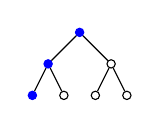
\begin{tikzpicture}[baseline=-0.5ex, scale=0.4]
    \tikzset{every node/.style={draw, circle, inner sep=0.5pt, minimum size=3pt}}
    \node[fill=Blue, draw=Blue] (N4) at (-1.50, -2) {};
    \node[] (N5) at (-0.50, -2) {};
    \node[fill=Blue, draw=Blue] (N2) at (-1.00, -1) {};
    \node[] (N6) at (0.50, -2) {};
    \node[] (N7) at (1.50, -2) {};
    \node[] (N3) at (1.00, -1) {};
    \node[fill=Blue, draw=Blue] (N1) at (0.00, 0) {};
    \draw (N1) -- (N2);
    \draw (N2) -- (N4);
    \draw (N2) -- (N5);
    \draw (N1) -- (N3);
    \draw (N3) -- (N6);
    \draw (N3) -- (N7);
  \end{tikzpicture}
}
\newsavebox{\boxshapep}
\sbox{\boxshapep}{
  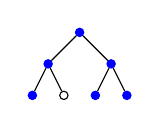
\begin{tikzpicture}[baseline=-0.5ex, scale=0.4]
    \tikzset{every node/.style={draw, circle, inner sep=0.5pt, minimum size=3pt}}
    \node[fill=Blue, draw=Blue] (N4) at (-1.50, -2) {};
    \node[] (N5) at (-0.50, -2) {};
    \node[fill=Blue, draw=Blue] (N2) at (-1.00, -1) {};
    \node[fill=Blue, draw=Blue] (N6) at (0.50, -2) {};
    \node[fill=Blue, draw=Blue] (N7) at (1.50, -2) {};
    \node[fill=Blue, draw=Blue] (N3) at (1.00, -1) {};
    \node[fill=Blue, draw=Blue] (N1) at (0.00, 0) {};
    \draw (N1) -- (N2);
    \draw (N2) -- (N4);
    \draw (N2) -- (N5);
    \draw (N1) -- (N3);
    \draw (N3) -- (N6);
    \draw (N3) -- (N7);
  \end{tikzpicture}
}
\newsavebox{\boxshapeq}
\sbox{\boxshapeq}{
  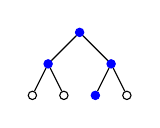
\begin{tikzpicture}[baseline=-0.5ex, scale=0.4]
    \tikzset{every node/.style={draw, circle, inner sep=0.5pt, minimum size=3pt}}
    \node[] (N4) at (-1.50, -2) {};
    \node[] (N5) at (-0.50, -2) {};
    \node[fill=Blue, draw=Blue] (N2) at (-1.00, -1) {};
    \node[fill=Blue, draw=Blue] (N6) at (0.50, -2) {};
    \node[] (N7) at (1.50, -2) {};
    \node[fill=Blue, draw=Blue] (N3) at (1.00, -1) {};
    \node[fill=Blue, draw=Blue] (N1) at (0.00, 0) {};
    \draw (N1) -- (N2);
    \draw (N2) -- (N4);
    \draw (N2) -- (N5);
    \draw (N1) -- (N3);
    \draw (N3) -- (N6);
    \draw (N3) -- (N7);
  \end{tikzpicture}
}
\newsavebox{\boxshaper}
\sbox{\boxshaper}{
  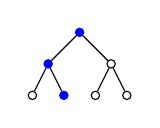
\begin{tikzpicture}[baseline=-0.5ex, scale=0.4]
    \tikzset{every node/.style={draw, circle, inner sep=0.5pt, minimum size=3pt}}
    \node[] (N4) at (-1.50, -2) {};
    \node[fill=Blue, draw=Blue] (N5) at (-0.50, -2) {};
    \node[fill=Blue, draw=Blue] (N2) at (-1.00, -1) {};
    \node[] (N6) at (0.50, -2) {};
    \node[] (N7) at (1.50, -2) {};
    \node[] (N3) at (1.00, -1) {};
    \node[fill=Blue, draw=Blue] (N1) at (0.00, 0) {};
    \draw (N1) -- (N2);
    \draw (N2) -- (N4);
    \draw (N2) -- (N5);
    \draw (N1) -- (N3);
    \draw (N3) -- (N6);
    \draw (N3) -- (N7);
  \end{tikzpicture}
}
\newsavebox{\boxshapes}
\sbox{\boxshapes}{
  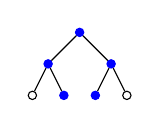
\begin{tikzpicture}[baseline=-0.5ex, scale=0.4]
    \tikzset{every node/.style={draw, circle, inner sep=0.5pt, minimum size=3pt}}
    \node[] (N4) at (-1.50, -2) {};
    \node[fill=Blue, draw=Blue] (N5) at (-0.50, -2) {};
    \node[fill=Blue, draw=Blue] (N2) at (-1.00, -1) {};
    \node[fill=Blue, draw=Blue] (N6) at (0.50, -2) {};
    \node[] (N7) at (1.50, -2) {};
    \node[fill=Blue, draw=Blue] (N3) at (1.00, -1) {};
    \node[fill=Blue, draw=Blue] (N1) at (0.00, 0) {};
    \draw (N1) -- (N2);
    \draw (N2) -- (N4);
    \draw (N2) -- (N5);
    \draw (N1) -- (N3);
    \draw (N3) -- (N6);
    \draw (N3) -- (N7);
  \end{tikzpicture}
}
\newsavebox{\boxshapet}
\sbox{\boxshapet}{
  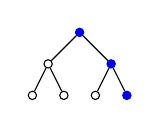
\begin{tikzpicture}[baseline=-0.5ex, scale=0.4]
    \tikzset{every node/.style={draw, circle, inner sep=0.5pt, minimum size=3pt}}
    \node[] (N4) at (-1.50, -2) {};
    \node[] (N5) at (-0.50, -2) {};
    \node[] (N2) at (-1.00, -1) {};
    \node[] (N6) at (0.50, -2) {};
    \node[fill=Blue, draw=Blue] (N7) at (1.50, -2) {};
    \node[fill=Blue, draw=Blue] (N3) at (1.00, -1) {};
    \node[fill=Blue, draw=Blue] (N1) at (0.00, 0) {};
    \draw (N1) -- (N2);
    \draw (N2) -- (N4);
    \draw (N2) -- (N5);
    \draw (N1) -- (N3);
    \draw (N3) -- (N6);
    \draw (N3) -- (N7);
  \end{tikzpicture}
}
\newsavebox{\boxshapeu}
\sbox{\boxshapeu}{
  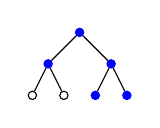
\begin{tikzpicture}[baseline=-0.5ex, scale=0.4]
    \tikzset{every node/.style={draw, circle, inner sep=0.5pt, minimum size=3pt}}
    \node[] (N4) at (-1.50, -2) {};
    \node[] (N5) at (-0.50, -2) {};
    \node[fill=Blue, draw=Blue] (N2) at (-1.00, -1) {};
    \node[fill=Blue, draw=Blue] (N6) at (0.50, -2) {};
    \node[fill=Blue, draw=Blue] (N7) at (1.50, -2) {};
    \node[fill=Blue, draw=Blue] (N3) at (1.00, -1) {};
    \node[fill=Blue, draw=Blue] (N1) at (0.00, 0) {};
    \draw (N1) -- (N2);
    \draw (N2) -- (N4);
    \draw (N2) -- (N5);
    \draw (N1) -- (N3);
    \draw (N3) -- (N6);
    \draw (N3) -- (N7);
  \end{tikzpicture}
}
\newsavebox{\boxshapev}
\sbox{\boxshapev}{
  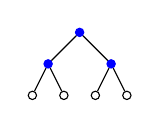
\begin{tikzpicture}[baseline=-0.5ex, scale=0.4]
    \tikzset{every node/.style={draw, circle, inner sep=0.5pt, minimum size=3pt}}
    \node[] (N4) at (-1.50, -2) {};
    \node[] (N5) at (-0.50, -2) {};
    \node[fill=Blue, draw=Blue] (N2) at (-1.00, -1) {};
    \node[] (N6) at (0.50, -2) {};
    \node[] (N7) at (1.50, -2) {};
    \node[fill=Blue, draw=Blue] (N3) at (1.00, -1) {};
    \node[fill=Blue, draw=Blue] (N1) at (0.00, 0) {};
    \draw (N1) -- (N2);
    \draw (N2) -- (N4);
    \draw (N2) -- (N5);
    \draw (N1) -- (N3);
    \draw (N3) -- (N6);
    \draw (N3) -- (N7);
  \end{tikzpicture}
}
\newsavebox{\boxshapew}
\sbox{\boxshapew}{
  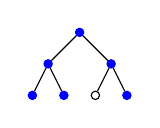
\begin{tikzpicture}[baseline=-0.5ex, scale=0.4]
    \tikzset{every node/.style={draw, circle, inner sep=0.5pt, minimum size=3pt}}
    \node[fill=Blue, draw=Blue] (N4) at (-1.50, -2) {};
    \node[fill=Blue, draw=Blue] (N5) at (-0.50, -2) {};
    \node[fill=Blue, draw=Blue] (N2) at (-1.00, -1) {};
    \node[] (N6) at (0.50, -2) {};
    \node[fill=Blue, draw=Blue] (N7) at (1.50, -2) {};
    \node[fill=Blue, draw=Blue] (N3) at (1.00, -1) {};
    \node[fill=Blue, draw=Blue] (N1) at (0.00, 0) {};
    \draw (N1) -- (N2);
    \draw (N2) -- (N4);
    \draw (N2) -- (N5);
    \draw (N1) -- (N3);
    \draw (N3) -- (N6);
    \draw (N3) -- (N7);
  \end{tikzpicture}
}
\newsavebox{\boxshapex}
\sbox{\boxshapex}{
  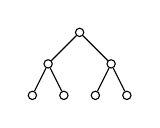
\begin{tikzpicture}[baseline=-0.5ex, scale=0.4]
    \tikzset{every node/.style={draw, circle, inner sep=0.5pt, minimum size=3pt}}
    \node[] (N4) at (-1.50, -2) {};
    \node[] (N5) at (-0.50, -2) {};
    \node[] (N2) at (-1.00, -1) {};
    \node[] (N6) at (0.50, -2) {};
    \node[] (N7) at (1.50, -2) {};
    \node[] (N3) at (1.00, -1) {};
    \node[] (N1) at (0.00, 0) {};
    \draw (N1) -- (N2);
    \draw (N2) -- (N4);
    \draw (N2) -- (N5);
    \draw (N1) -- (N3);
    \draw (N3) -- (N6);
    \draw (N3) -- (N7);
  \end{tikzpicture}
}
\newsavebox{\boxshapey}
\sbox{\boxshapey}{
  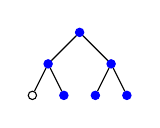
\begin{tikzpicture}[baseline=-0.5ex, scale=0.4]
    \tikzset{every node/.style={draw, circle, inner sep=0.5pt, minimum size=3pt}}
    \node[] (N4) at (-1.50, -2) {};
    \node[fill=Blue, draw=Blue] (N5) at (-0.50, -2) {};
    \node[fill=Blue, draw=Blue] (N2) at (-1.00, -1) {};
    \node[fill=Blue, draw=Blue] (N6) at (0.50, -2) {};
    \node[fill=Blue, draw=Blue] (N7) at (1.50, -2) {};
    \node[fill=Blue, draw=Blue] (N3) at (1.00, -1) {};
    \node[fill=Blue, draw=Blue] (N1) at (0.00, 0) {};
    \draw (N1) -- (N2);
    \draw (N2) -- (N4);
    \draw (N2) -- (N5);
    \draw (N1) -- (N3);
    \draw (N3) -- (N6);
    \draw (N3) -- (N7);
  \end{tikzpicture}
}
\newsavebox{\boxshapez}
\sbox{\boxshapez}{
  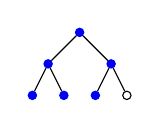
\begin{tikzpicture}[baseline=-0.5ex, scale=0.4]
    \tikzset{every node/.style={draw, circle, inner sep=0.5pt, minimum size=3pt}}
    \node[fill=Blue, draw=Blue] (N4) at (-1.50, -2) {};
    \node[fill=Blue, draw=Blue] (N5) at (-0.50, -2) {};
    \node[fill=Blue, draw=Blue] (N2) at (-1.00, -1) {};
    \node[fill=Blue, draw=Blue] (N6) at (0.50, -2) {};
    \node[] (N7) at (1.50, -2) {};
    \node[fill=Blue, draw=Blue] (N3) at (1.00, -1) {};
    \node[fill=Blue, draw=Blue] (N1) at (0.00, 0) {};
    \draw (N1) -- (N2);
    \draw (N2) -- (N4);
    \draw (N2) -- (N5);
    \draw (N1) -- (N3);
    \draw (N3) -- (N6);
    \draw (N3) -- (N7);
  \end{tikzpicture}
}
\begin{tikzpicture}[yscale=1.8,xscale=2.8]
\newcommand{\edgespathclr}{Blue}
\newcommand{\edgesclr}{gray}
\coordinate (1) at (2.00, 1);
\coordinate (1-3) at (0.00, 2);
\coordinate (1-2-3-5-7) at (0.80, 5);
\coordinate (1-2) at (4.00, 2);
\coordinate (1-2-3-4) at (4.00, 4);
\coordinate (1-3-6-7) at (0.00, 4);
\coordinate (1-2-3-4-5-6-7) at (2.00, 7);
\coordinate (1-3-6) at (1.00, 3);
\coordinate (1-2-4-5) at (3.20, 4);
\coordinate (1-2-3-4-5) at (2.40, 5);
\coordinate (1-2-3-4-7) at (3.20, 5);
\coordinate (1-2-3-7) at (1.60, 4);
\coordinate (1-2-3-5) at (2.40, 4);
\coordinate (1-2-3-4-6) at (4.00, 5);
\coordinate (1-2-4) at (4.00, 3);
\coordinate (1-2-3-4-6-7) at (4.00, 6);
\coordinate (1-2-3-6) at (0.80, 4);
\coordinate (1-2-5) at (3.00, 3);
\coordinate (1-2-3-5-6) at (1.60, 5);
\coordinate (1-3-7) at (0.00, 3);
\coordinate (1-2-3-6-7) at (0.00, 5);
\coordinate (1-2-3) at (2.00, 3);
\coordinate (1-2-3-4-5-7) at (2.67, 6);
\coordinate (empty) at (2.00, 0);
\coordinate (1-2-3-5-6-7) at (0.00, 6);
\coordinate (1-2-3-4-5-6) at (1.33, 6);
\foreach\a/\b in {
1-2-3-4/1-2-3-4-6, 1-2-3-4-7/1-2-3-4-5-7, 1-2-3-4-5-7/1-2-3-4-5-6-7, 1-2-3-4-5/1-2-3-4-5-6, 1-2-3-5/1-2-3-4-5, 1-3/1-3-6, 1-3-6-7/1-2-3-6-7, 1/1-2, 1-2-3/1-2-3-7, 1-2-3/1-2-3-5, 1-2-4/1-2-4-5, 1-2-3-7/1-2-3-6-7, 1-2-3-5/1-2-3-5-6, 1-2-3-5-6-7/1-2-3-4-5-6-7, 1-2-3/1-2-3-6, 1-2-3-4/1-2-3-4-5, 1-2/1-2-3, 1-3-6/1-3-6-7, 1-2-3-6-7/1-2-3-5-6-7, 1-2-3-7/1-2-3-5-7, 1-2-3-4-5/1-2-3-4-5-7, 1-2-3-5-6/1-2-3-5-6-7, 1-2-4-5/1-2-3-4-5, 1-2-3-4-6-7/1-2-3-4-5-6-7, 1-2-3-4-6/1-2-3-4-6-7, 1-2-5/1-2-4-5, 1-3/1-2-3}{
    \draw[\edgesclr] (\a) -- (\b);
}
\draw[\edgesclr] (1-2) -- (1-2-4);
\foreach\a/\b in {
1/1-3, 1-2-3-4-5-6/1-2-3-4-5-6-7, 1-2-4-5/1-2-4, 1-2-5/1-2-3-5, 1-2-3-4-7/1-2-3-4-6-7, 1-3-7/1-3-6-7, 1-2-3-7/1-2-3, 1-3/1-3-7, 1-2-3-6-7/1-2-3-7, 1-2-3-5/1-2-3-5-7, 1-2-3-4-5-6-7/1-2-3-4-5-7, 1-3-6-7/1-3-6, 1-2-3-6/1-2-3-6-7, 1-2-3-5-6-7/1-2-3-5-6, 1-2-3/1-2, 1-3-6/1-2-3-6, 1-2-3-5-7/1-2-3-5-6-7, 1-2-3-4/1-2-3-4-7, 1-2-3-4-5/1-2-4-5, 1-2/1-2-5, 1-2-3-5-6/1-2-3-4-5-6, 1-2-4/1-2-3-4, 1-2-3-4-6-7/1-2-3-4-6, 1-2-3-4-5-7/1-2-3-4-5, empty/1}{
    \draw[\edgespathclr, ultra thick] (\a) -- (\b);
}
\node[draw, fill=white, inner sep=2pt, rounded corners=2pt] at (1) {\usebox{\boxshapea}};
\node[draw, fill=white, inner sep=2pt, rounded corners=2pt] at (1-3) {\usebox{\boxshapeb}};
\node[draw, fill=white, inner sep=2pt, rounded corners=2pt] at (1-2-3-5-7) {\usebox{\boxshapec}};
\node[draw, fill=white, inner sep=2pt, rounded corners=2pt] at (1-2) {\usebox{\boxshaped}};
\node[draw, fill=white, inner sep=2pt, rounded corners=2pt] at (1-2-3-4) {\usebox{\boxshapee}};
\node[draw, fill=white, inner sep=2pt, rounded corners=2pt] at (1-3-6-7) {\usebox{\boxshapef}};
\node[draw, fill=white, inner sep=2pt, rounded corners=2pt] at (1-2-3-4-5-6-7) {\usebox{\boxshapeg}};
\node[draw, fill=white, inner sep=2pt, rounded corners=2pt] at (1-3-6) {\usebox{\boxshapeh}};
\node[draw, fill=white, inner sep=2pt, rounded corners=2pt] at (1-2-4-5) {\usebox{\boxshapei}};
\node[draw, fill=white, inner sep=2pt, rounded corners=2pt] at (1-2-3-4-5) {\usebox{\boxshapej}};
\node[draw, fill=white, inner sep=2pt, rounded corners=2pt] at (1-2-3-4-7) {\usebox{\boxshapek}};
\node[draw, fill=white, inner sep=2pt, rounded corners=2pt] at (1-2-3-7) {\usebox{\boxshapel}};
\node[draw, fill=white, inner sep=2pt, rounded corners=2pt] at (1-2-3-5) {\usebox{\boxshapem}};
\node[draw, fill=white, inner sep=2pt, rounded corners=2pt] at (1-2-3-4-6) {\usebox{\boxshapen}};
\node[draw, fill=white, inner sep=2pt, rounded corners=2pt] at (1-2-4) {\usebox{\boxshapeo}};
\node[draw, fill=white, inner sep=2pt, rounded corners=2pt] at (1-2-3-4-6-7) {\usebox{\boxshapep}};
\node[draw, fill=white, inner sep=2pt, rounded corners=2pt] at (1-2-3-6) {\usebox{\boxshapeq}};
\node[draw, fill=white, inner sep=2pt, rounded corners=2pt] at (1-2-5) {\usebox{\boxshaper}};
\node[draw, fill=white, inner sep=2pt, rounded corners=2pt] at (1-2-3-5-6) {\usebox{\boxshapes}};
\node[draw, fill=white, inner sep=2pt, rounded corners=2pt] at (1-3-7) {\usebox{\boxshapet}};
\node[draw, fill=white, inner sep=2pt, rounded corners=2pt] at (1-2-3-6-7) {\usebox{\boxshapeu}};
\node[draw, fill=white, inner sep=2pt, rounded corners=2pt] at (1-2-3) {\usebox{\boxshapev}};
\node[draw, fill=white, inner sep=2pt, rounded corners=2pt] at (1-2-3-4-5-7) {\usebox{\boxshapew}};
\node[draw, fill=white, inner sep=2pt, rounded corners=2pt] at (empty) {\usebox{\boxshapex}};
\node[draw, fill=white, inner sep=2pt, rounded corners=2pt] at (1-2-3-5-6-7) {\usebox{\boxshapey}};
\node[draw, fill=white, inner sep=2pt, rounded corners=2pt] at (1-2-3-4-5-6) {\usebox{\boxshapez}};
\end{tikzpicture}
